\documentclass[authoryear, preprint, review, 12pt]{elsarticle}

\usepackage{lineno}
\usepackage[USenglish]{babel}
\usepackage[utf8x]{inputenc}
\usepackage{amsmath}
\usepackage{amssymb}
\usepackage{amsthm}
\usepackage{graphicx}
\usepackage{subfig}
\usepackage{microtype} 
\usepackage{bm}
\usepackage{verbatim}
\usepackage{adjustbox}
\usepackage[para,online,flushleft]{threeparttable}
\usepackage[table,xcdraw,dvipsnames]{xcolor}
\usepackage{booktabs,multirow}
\usepackage{array, longtable}
\usepackage[font=normalsize]{caption}
\usepackage{afterpage}
\usepackage{tabularx}
\usepackage{float}
\usepackage{color}
\usepackage{fullpage}
\usepackage{setspace}
\usepackage{csquotes}
\usepackage{dcolumn}
\usepackage[notablist,nofiglist]{endfloat}
\usepackage[final]{pdfpages}
\usepackage[colorlinks=true, allcolors=Blue]{hyperref}
\usepackage[colorinlistoftodos]{todonotes}

\usepackage{rotating}
\usepackage{pdflscape}

\DeclareDelayedFloatFlavor{sidewaystable}{table}
\DeclareDelayedFloatFlavour*{longtable}{table}
\DeclareDelayedFloatFlavour*{longsidewaystable}{table}

\usepackage{natbib}

\renewcommand{\thetable}{\arabic{table}}

\journal{European Economic Review}

\begin{document}

\begin{frontmatter}
\title{Little lies \\ Math performance and cheating in primary schools in Congo}

\end{frontmatter}

\section{Introduction}
In everyday life we often observe dishonesty and cheating: citizens evade taxes, drivers park in forbidden spaces, viewers illegally download content from the Internet, students copy in written exams, employees call in sick when they are not ill, users enjoy public transportation as free riders. In an effort to limit dishonesty, governments apply fiscal inspections, city councils hire parking inspectors, media companies and content distributors implement technological innovations to hinder copyright infringements, professors employ Ph.D. students as invigilators during exams, official doctors may check up on sick leave, and bus companies hire ticket checkers\footnote{For extensive surveys on behavioral mechanisms and psychological causes affecting dishonesty, see \cite{ma06} and \cite{jacobsen2018we}.}. 
    
Cheating and lying are generally seen as anti-social behaviors since being unable to trust others' word and behavior bears substantial economic and social costs and destroys the social fabric of human coexistence. In this perspective, cheaters are perceived as social outcasts which try to compensate their lack of talent or effort with unfair behaviors, thus cheating can be better understood within a cost-benefit framework \citep{gtw13,g05}. 

However, there are also plenty of counterexamples: on the one hand, there are situations and micro-cultures in which cheating is sometimes seen as a proxy of smartness, such as gang and street culture \citep{b13} or even business culture \citep{cfm14}; on the other hand, psychological empirical research \citep{vasek1986lying,exl11,el13} shows that lying in children is correlated with the development of cognitive skills, therefore it can be a good predictor of future school achievements. 

An extensive experimental literature studies dishonesty in Psychology \citep{gl15,wsr03,ph99} and Economics \citep{pate2018temptation, kg17,ruffle2017clever,ariely2015true,ff13, hurkens2009,maa08,g05}. In both fields, a number of papers \citep{cantin2016executive,maggian2016social,gl15,el13,ding2014elementary,bucciol2011temptation,bucciol2011luck,talwar2007lying} explicitly focuses on children lying behavior, investigating the influence of different factors such as: age, gender, social preferences and second-order belief understanding. 

A vast and detailed taxonomy of lies has been established and a panoply of different tests, tasks and situations have been devised in order to study every different shades of lies.\cite{erat2012white} through a dice rolling experiment distinguish between \textit{Altruistic white lies} (when the lie harm the liar but help the other person), \textit{Pareto white lies} (when both sides earn more as a result of the lie\footnote{\cite{maggian2016social}, along the line of \cite{g05}, correctly points out that the gain for both sides is not needed in order to define a \textit{White} lie as a \textit{Pareto} one since any lie which increases the utility of the \enquote{partner} without diminishing the utility of the \enquote{player} will perfectly fit the definition.}), \textit{Selfish black lies} (when the lie help the liar at the expenses of the other person) and \textit{Spiteful black lies} (when both sides looses as a result of the lie).

Our paper delves within this debate by providing a novel contribution on the relation existing between school performance (with a specific focus on math scores), cheating and pro-social attitudes among primary school children, by adopting a slightly modified version of the dice-rolling task\footnote{As in \cite{ariely2015true}.}, in which no counterpart in the game is explicitly mentioned and the subject is required to report the outcome (thus possibly lying) under the direct scrutiny of the interviewer. 

Through a cross-section analysis of 170 children randomly selected\footnote{See Section \ref{subsec: Data and variables} for a description of sampling procedures. Please note that due to some missing information in a handful of school reports, the actual number of observations in the regression tables can be smaller than 170.} in 10 primary schools in the outskirts of Goma, we are able to show that \textit{cheating behavior} is a stable and specific characteristic of the sample and that it is strongly predicted by both \textit{Math} and \textit{Total} scores, recorded in school reports, and negatively correlated with an experimental measure of \textit{Altruism}. Finally we give evidence that math-skilled pupils tend to cheat more when rewards from cheating are higher, thus suggesting that these pupils are better equipped to rapidly identify costs and benefits of cheating and act consequently.

To achieve this aim, the paper exploits data produced in a Lab-in-the-Field Experiment we conducted, with two other colleagues\footnote{Names removed in the anonymous version for referees.}, in the Democratic Republic of Congo (March 2016 and May 2017), originally devised to measure the effectiveness of a distance adoption program implemented by AVSI\footnote{See \url{https://www.avsi.org/en/}.}, an Italian NGO. The nature of the dataset allows us to introduce a twofold original contribution: on the one hand, we can account for possible unobserved heterogeneity in cheating levels \textit{before} Total and Math performance were recorded (i.e. in the previous school year); on the other hand, we can control for a measure of altruism (also recorded in the previous school year), to account for individual heterogeneity in pro-social preferences.

Since our original experimental framework involves a dice rolling task (DRT, henceforth) to be performed by a primary school child under the direct sight of an adult interviewer, in contrast with the original setting proposed by \cite{ff13}, we are in the best position to test whether cheating is a prominent behaviour within our sample. In other words, if we are able to detect a significant level of cheating in our experiment, \textit{a fortiori} we would have observed an even larger level if the experiment were performed in the standard format.  

Furthermore, since in our experimental protocol the child is aware that in the DRT no counterpart (i.e a fellow pupil, as it is the case, conversely, in the Dictator Game) is harmed by his/her lie, the only effect being that the interviewer has to disburse a larger number of biscuits, we are able to test whether cheating is conceived as an anti-social behaviour \textit{per se}.

Finally, by studying cheating patterns (i.e. the relations between cheating behaviour and the gain from cheating in each individual dice draw) we are able to test whether math related school performance significantly differs, in this respect, from generic school performance (as measured by \textit{Total score}).

The paper is organized as follows: Section \ref{sec:ResDes} presents the research design and experimental methods, Section \ref{sec:Empiric} outlines the estimation techniques, Section \ref{sec:results} provides main results and robustness checks, Section \ref{sec:revcause} deals with potential reverse causation, Section \ref{sec:cheatpattern} investigates cheating patterns, Section \ref{sec:conclusion} discusses the main findings and concludes the paper.

\section{Research Design}
\label{sec:ResDes}

%subsection{Experimental procedures}
\subsection{The sample}
\label{subsec:sample}
The experimental procedure involves the administration of a questionnaire, including a set of incentivized tasks, on a sample of 170 children from 28 different classes, across ten primary schools in the outskirts of Goma, a city located in the troubled North Kivu province of the Democratic Republic of Congo. The questionnaire has been administered twice, in two school years (2015/16 and 2016/17), at the end of the second term of each school year\footnote{The questionnaire was administered in paper-and-pencil, the first time in late March 2016 and the second in early May 2017.}. Thanks to the time structure of the data collection protocol, we are able to exploit the time interval (around 13 months) between the two observations, to account for potential \textit{ex ante} individual heterogeneity in cheating behaviour, and to investigate the existence of reverse causation.

The sample used in this paper consists of a number of \enquote{control} children that have been randomly chosen to match, w.r.t. to school, class, age and gender, a given number of children supported by AVSI distance adoption program (SAD), on the basis of a \enquote{vulnerability scale} computed (taking into account both the children and the household situation) by the NGO.
For each treated child, we asked each school to randomly select two children, matching age and gender and attending the same class, to provide a control group for the evaluation of the program. Since SAD children are randomly assigned to different classes by school headmaster, for the purpose of this paper, we well may consider that no influence of the support program comes into play and our sample of \enquote{control} children to be representative of the entire population of non-treated children in the selected 10 primary schools in Goma. 

From the initial resulting number of 188 children, 18 children have been excluded from the analysis since they failed the class in 2015/2016 and had to repeat the same grade in 2016/2017, thus their school performance in 2016/2017 could not be compared with the rest of the sample. The final sample consists of 170 children. Descriptive statistics of our sample's individual characteristics are shown in Table \ref{tab:sumstat}. 

\subsection{Experimental procedures}
\label{subsec:ExpProc}
Incentivized tasks in behavioral and experimental economics are usually performed by using money as incentive. However, both ethical concerns, given the subjects' age (ranging from 6 to 16), and the geopolitical conditions of the area suggested not to handing out (even small amount of) money to the interviewed children. Following the suggestions of NGOs working in the area, we resorted to use packets of biscuits as incentive goods\footnote{NGO's staff identified the biscuits brand and type \enquote{Cremica Glucose Biscuits} whose packaging is best known and which is most appreciated by children. Local sources informed us that these biscuits are also used as means of exchange among school children, thus minimizing possible satiation issues involved when using food as a reward in experiments.}. 

Parents provided active consent after being adequately informed before the experiment took place. Moreover, both the interviewers and the good used to reward the participants (biscuits) were presented in advance to children and parents by the school headmasters. Questionnaires have been administered by twenty-seven interviewers purposely recruited among students of the local university in Goma. Interviewers were independent from both the schoolteachers and the NGO and were previously unknown to children.

Pupils were interviewed one at a time, by one interviewer sitting in front of one pupil, in order to ensure that instructions were fully understood. Nobody else was allowed to stay in the room during the experiment. After introducing him/herself to the child, the interviewer set the table by putting a picture of schoolchildren (taken in a different school, in the same region, not included in the analysis) in front of the child as an help to visualize his/her anonymous partner for the Dictator Game.   

Thanks to the cooperation of schools' headmasters, children involved in the experiment were gathered together in the school's courtyard. After a child  completed the questionnaire, he/she was allowed to return home, thus avoiding that he/she could talk about the experiment to other children still waiting to be interviewed.
All the tasks included in the questionnaire were played in an anonymous double blind setting: children were randomly assigned a code; the NGO staff held records about the matching between individual names and codes, but could not access individual outcome data; the research team could access individual outcome data, matched with anonymous codes, but could not access individual names\footnote{For further details on the experimental procedures see also [Authors 2017].}.

Each task yields a payoff in terms of packets of biscuits, depending on children's choices. At the end of the questionnaire, only one of the incentivized tasks is drawn (through a die roll) and actually rewarded: in this way, children are supposedly putting the same effort on every task.

\subsection{Incentivized tasks: Dice Rolling and Dictator}
\label{subsec:IncTask}
The incentivized tasks relevant to this paper are described below:
\begin{itemize}
\item \textit{Dice rolling task}. This task, originally developed by \citet{ff13} and applied in different contexts \citep[e.g.][]{ariely2015true}, exploits the statistical properties of random dice rolls to make inference about mind cheating (i.e. misreporting of chosen outcomes) in both children and adults.
In our experiment, we slightly modified the original version of the task in order to make it easier for children to understand. Instead of using a single die (with the \textit{ex ante} choice being between the top or bottom side), the child is provided with a couple of fair dice (one red and one blue) and asked by the interviewer to perform twenty rolls. Before every roll, the child has to decide in his/her mind which of the two dice (either the red or the blue one) he/she will choose. After observing the outcome of the roll, he/she communicates his/her own choice to the interviewer that takes note of the choice in the questionnaire form. At the end of all 20 rolls, one is randomly chosen and selected for being rewarded (in case the dice task is drawn as the task to be rewarded) at the end of the interview. The choice is not declared before the roll, therefore the child has always the incentive and the opportunity to deviate from his/her original choice and simply choose the highest outcome between the two dice. If the child's reporting is sincere, children should, on average, have chosen the highest die in each roll half of the times and the average outcome of the chosen dice should approximate the expected value of the series, since any \textit{ex ante} choice strategy is independent of the outcome. If, on the contrary, the child chose the highest die more than 50\% of the times and/or the mean of the chosen outcomes exceeds the expected value of the series of rolls, it is likely that the child may have misreported (thus cheating) his/her choices to maximize his/her payoff. Clearly, the statistical properties of this task hold on average for the sample but not necessarily at the individual level because of the small number (equal to 20) of rolls\footnote{Please refer to \citet{ariely2015true} for further details on the statistical properties of the DRT.}.

Our main cheating indicator \textit{(MaxChoice)}, is computed as the proportion of maximum values stated by children over their total number of rolls (net of ties)\footnote{Given the presence of ties, the number of relevant rolls may differ across children.}. A second measure of cheating (\textit{MeanRoll}) is the difference between the average of the 20 dice values he/she has chosen and the total average computed over of his/her series of 20 rolls of two (one blue, one red) dice\footnote{It must be noted that because our subjects (children) roll two fair dice, the outcomes of the blue die is independent from the outcome of the red die. For this reason, differently from \citet{ariely2015true,ff13} total average can also be different from one child to another one: therefore, our indicator adjusts for individual variation and provides a more accurate aggregate indicator of cheating behavior.}. 

As already stated in the introduction, our experimental framework differs from other papers using DRT \citep{shalvi2011justified, ff13, ariely2015true, houser2013perceptions, gachter2016intrinsic} in two main respects: firstly the task was performed by a primary school child under the direct sight of an adult interviewer, thus imposing a rather high \enquote{psychological cost} of lying given on the subject due to the fear of being caught; secondly, and differently from what happen in the Dictator Game, we make the child explicitly aware that in the DRT no counterpart (i.e a fellow pupil) is harmed by his/her lie\footnote{The only effect being that the interviewer has to disburse a larger number of biscuits, thus in a sense we may consider our experimental protocol to target a very specific sub-type of \textit{Pareto White} lie.}. Through these two small changes in the protocol we are therefore able to test whether cheating is a prominent behaviour within our sample and whether it is conceived as an anti-social behaviour \textit{per se}, irrespective of the consequences. 

\item \textit{Dictator Game}. The questionnaire includes a modified version of the Dictator Game (DG, henceforth) \citep{kahneman1986} in which the interviewed child acts as a Proponent, being endowed with five packets of biscuits and matched to an anonymous child who has received no endowment.
The task requires the child to choose if and how to split the packets of biscuits he/she received between him/herself and the anonymous, randomly assigned, partner\footnote{The interviewer stated to the subject that he/she had been randomly matched with an anonymous child among those depicted in a photo (in which about 40 primary school children from another school, not part of the analysis, were visible). The priming aimed at stressing that the \enquote{partner} was a child with similar characteristics compared to the subject: not richer or poorer, within an analogous age range. Both males and females children were depicted in the photo to avoid any \textit{inter}-gender or \textit{intra}-gender bias.}. The non shared amount corresponds to the individual pay-off in case the DG is drawn as the task to be rewarded. Within a pure game theoretical framework with self-interested agents, the Proponent is expected to retain the entire endowment for him/herself. Deviations from the \emph{selfish} equilibrium solution in the DG can thus measure empathy, altruism and/or pure generosity \citep{forsythe1994,camerer2003,guala2010paradigmatic}. We use the proportion of the initial endowment of packaged biscuits shared with the other child as an indicator of \textit{Altruism}.
\end{itemize}

\subsection{School reports}
\label{sub:schoolreport}
In this paper we employ the pupil's performance in Math (Math score) as our main explanatory variable, while using the general school performance (Total score) as a robustness check.

We collected school reports for two school years (2015/16 and 2016/17). The school year in Congo begins in October and ends in June.  Results are recorded at the end of each term; in this paper we used 2\textsuperscript{nd} terms' results because they better matched the timing of administration of the questionnaire. School reports in Congo include a large number of scores, splitting subjects into topics and terms in smaller sub-periods\footnote{School reports for primary schools in Congo are very complex and exhaustive documents reporting for each child two intermediate marks plus a final score per each term in six main subjects/areas: Religion and Civic education, National Languages, French Language, Mathematics, Sciences, Arts. Math and Total score included in the analysis provided in this section both refer to the same term of 2016/17.}. Aggregate scores, by subject and term, are obtained by the sum of all the relevant sub-components. In order to make Total and Math scores comparable across grades and subjects, we harmonized scores by converting them as shares of the maximum numeric outcome achievable for each subject in any given grade.

\section{Empirical analysis}
\label{sec:Empiric}
\subsection{Estimation techniques}
\label{sec:estimation}

We estimate the relation between school performance and cheating behaviour through a cross-section analysis in which the main outcomes, namely the value of one of the cheating indicators in school year 2016/17, are predicted by the main independent variable, i.e. Math score. To estimate the effect on cheating (alternatively measured by either MaxChoice or MeanRoll) we estimate the following model:

\begin{equation}
\label{eq:model1}
\begin{split}
    Cheat_{i} &= \alpha + \beta SchoPer_{i} + \gamma Altruism_{i} + \delta Cheat (baseline)_{i} \\ 
                 &+ \sum\limits_{k=1}^K\rho_k Z_{ki} + \sum\limits_{j=1}^J\mu_j Dummies_{ji} + \epsilon_{i}
\end{split}
\end{equation}
 
where $i$ identifies pupils; $Cheat$ is the value of the cheating indicator in school year 2016/2017, $SchoPer$ is the main explanatory variable for school performance, alternatively measured by Math and Total score, $Altruism$ is the main explanatory variable for pro-social attitudes, $Z$ is a set of $K$ individual characteristics, such as gender and age, as well as the individual payoff obtained in the first experimental session in 2015/16, $Dummies$ is a set of $J$ dummies to control for invariant characteristics, such as pupils' school, grade of attendance, peer effects (as defined in Table \ref{tab:description}) and to control for the interviewer that administered the questionnaire; $\alpha$, $\beta$, $\gamma$, $\delta$, $\rho$, $\mu$ are the parameters to be estimated, while $\epsilon_{i}$ is the usual error term. 

When we estimate the effect of Math performance on MaxChoice, we adopt a GLM estimator for the binomial family with a logit link function \citep{papkewoolridge96}, to account for the fact that our  main cheating indicator is a share, hence it is bounded within 0 and 1; when we use the alternative cheating indicator, MeanRoll, we simply estimate the model through OLS, including robust standard errors.

Finally, in Section \ref{sec:cheatpattern} we investigate the pattern of dice outcome choices through the whole roll series, therefore our dependent variable is binary. In this case, to predict the probability of choosing the maximum outcome as a function of school performance ($SchoPer$), conditional on the observed difference between the two dice, we implement the following (interacted and fully saturated) logit model:

\[ Y_i,_r =
\begin{cases}
 1  & \quad \text{if pupil $i$ chooses maximum outcome between the two dice in roll $r$} \\
 0  & \quad \text{otherwise}\\
\end{cases}
\]

\begin{equation}\begin{split}
\label{eq:logit}
log\left(\frac{\pi_i,_r}{1-\pi_i,_r}\right) &= \alpha + \beta SchoPer_{i} + \gamma SchoPer_{i}\times High Dif_{ir} + \delta High Dif_{ir} \\ 
                  &+ \sum\limits_{k=1}^K\rho_k Z_{ki} + \sum\limits_{j=1}^J\mu_j Dummies_{ji} 
\end{split}\end{equation}

where
$\pi_i,_r$ is the probability that $Y_i,_r$ equals 1, $Y$ is the dependent variable, $SchoPer$ is the main explanatory variable for school performance, alternatively measured by Math and Total score, $High Dif_{ir}$ is the binary variable identifying \enquote{high} (absolute) differences (i.e. 4 or 5) between the two dice observed by pupil $i$ in roll $r$, $Z$ and $Dummies$ are defined as in Equation \ref{eq:model1} and $\alpha$, $\beta$, $\gamma$, $\delta$, $\rho$, $\mu$ are the parameters to be estimated. Standard errors are clustered at the individual level.

\subsection{Data and variables}
\label{subsec: Data and variables}
Data for our outcome indicators (MaxChoice and MeanRoll) as well as for our main explanatory variables (Math and Total score) and control variables (Female, Age, Payoff) refer to the school year 2016/17. Altruism and \enquote{baseline} cheating indicators (used as covariates) are measured in school year 2015/2016, i.e. roughly one year earlier. Further, Math and Total scores are collected in the second term of each school year and their values have been re-scaled in relative term to allow inter-class/inter-term comparability as explained in Section \ref{sub:schoolreport}\footnote{W.r.t. the experiment administration, school year 2015/16 refers to the first wave (Wave 1); school year 2016/17 refers to the second wave (Wave 2).}.

All variables included in the analysis are briefly described in Table \ref{tab:description}, while Table \ref{tab:sumstat} provides descriptive statistics. 

\begin{table}[!h]\centering \caption{Variables description}
\renewcommand*{\arraystretch}{1}
\begin{tabular}{l p{9.5cm}}\toprule
\textbf{Variable} 			& \textbf{Description} 			\\ \midrule
\textit{Behavioural indicators} & \\
MaxChoice 					& Proportion of maximum values in a given roll chosen by children over the total number of throws (excluding ties)						\\
MeanRoll 					& Difference between average reported outcome and expected values of individual dice rolls	\\
Altruism 					& Proportion of packets of biscuits sent to the anonymous respondent						\\
&\\
\textit{School performance indicators} & \\
Math score					& Score in Math in second term, harmonized by dividing \enquote{raw scores} resulting from official school reports by the maximum achievable points for term 2 \\
Total score					& Total score in term 2 (arithmetic sum of all individual subject scores, harmonized (same procedure described above) \\
&\\ \midrule
\textit{Dice roll patterns} & \\
High Dif 					& Binary variable equals to 1 when the absolute difference between red and blue dice observed outcomes in individual roll series is equal to 4 or 5. \\
Low Dif					& Binary variable equals to 1 when the absolute difference between red and blue dice observed outcomes in individual roll series is equal to 1, 2, or 3. Used as omitted reference category in regressions. \\
\textit{Individual characteristics}&			\\
Age 		 				& Self-reported pupil's age								\\
Female 						& Dummy variable equals to 1 if pupil is female	\\
&\\
\textit{Experiment characteristics}&			\\
Payoff                      & Payoff earned by child at the end of the first wave (September 2017) \\
Dummies: & \\
- Schools              & Dummy variables identifying pupil's schools \\
- Grades              & Dummy variables identifying pupil's grades \\
- Peer effects  & Dummy variables identifying pupil's grades within each school \\
- Interviewers         & Dummy variables identifying interviewers \\
\bottomrule
\end{tabular} 
\label{tab:description}
\end{table}

% Dice Diff=$k$ 					& Absolute difference between red and blue dice observed outcomes in individual roll series, for $k$ possible values, with 0 $\le k \le 5, k\in\mathbb{N}$ \\
\begin{table} \centering
	\caption{Summary statistics, school year 2016/2017}
	\begin{threeparttable}
		\centering
		\begin{tabular}{l*{5}{D{.}{.}{-1}}} 
			\toprule
	&       Mean&          SD&      Min 	&		Max			& Obs	\\
			\toprule			
\textit{Behavioural indicators} &&&&& \\
MaxChoice           &       0.676&       0.234&       0.000&       1.000&         170\\
MaxChoice, baseline &       0.648&       0.217&       0.176&       1.000&         170\\
MeanRoll            &       0.356&       0.487&      -1.075&       1.250&         170\\
MeanRoll, baseline  &       0.296&       0.455&      -0.775&       1.300&         170\\
Altruism, baseline  &       0.412&       0.167&       0.000&       0.800&         170\\ 
\midrule
\textit{School performance indicators} &&&&& \\
Math score          &       0.638&       0.150&       0.305&       0.970&         169\\
Total score         &       0.627&       0.116&       0.332&       0.866&         169\\
\midrule
\textit{Control variables} &&&&& \\ 
Female              &       0.500&       0.501&       0.000&       1.000&         170\\
Age                 &       8.729&       1.459&       6.000&      13.000&         170\\
Payoff              &       2.147&       1.442&       0.000&       6.000&         170\\
\bottomrule
\end{tabular}
\begin{tablenotes}
\footnotesize
\textit{Notes:} Baseline refers to school year 2015/2016. The sample includes only children that were not repeating their grade due to failure in school year 2015/2016.
\end{tablenotes}
\end{threeparttable}
\label{tab:sumstat}
\end{table}

The final sample included in the analysis presented in the next Section accrues to 170 pupils, randomly chosen in 28 different classes, across 10 primary schools in Goma.

\section{Results}
\label{sec:results}

\subsection{Descriptive analysis}
\label{subsec:Descriptive}
Despite the experimental framework was rather unfavourable to cheating - children had to perform the task and report their choice in front of an adult - cheating is the prevailing behaviour in our sample, as shown by the sample means of both indicators (MaxChoice and MeanRoll) in Table \ref{tab:sumstat}. A t-test on the mean value of MaxChoice shows that it is significantly different from 0.5 (p$<$0.001), which is the aggregate probability of randomly choosing ex-ante the die showing the highest value of the couple. The same analysis performed on the mean value of MeanRoll show that its value is positive and significantly different from zero (p$<$0.001)\footnote{The same results hold for both baseline cheating indicators, as recorded in s.y. 2015/16.}.
These results are graphically depicted by the histograms in Figure \ref{fig:cheating}, where the distributions of both MaxChoice and MeanRoll are skewed to the right of the dashed lines (one centred on 0.5, the other on 0), representing the mean of an hypothetical random (i.e. non cheating) behaviour. On the contrary, both Math Score and Total Score display an almost normal distribution centred on values around 0.6 (see Figure \ref{fig:performance}).

\begin{figure}[!h]
  \centering
	\includegraphics[width=.8\linewidth]{figures/hist_meanrollANDmaxchoice.eps} \caption{Distribution of MaxChoice and MeanRoll indicators, s.y. 2016/17.}\label{fig:cheating}
\end{figure}

\begin{figure}[!h]
  \centering
	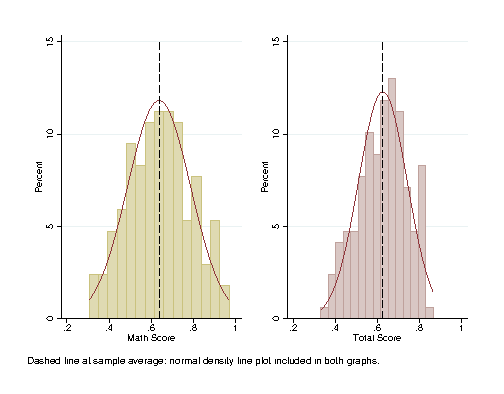
\includegraphics[width=.8\linewidth]{figures/hist_mathANDtot.eps} \caption{Distribution of Math and Total score outcomes, s.y. 2016/17.}\label{fig:performance}
\end{figure}

Looking for possible determinants of individual variation in cheating behaviour, and in particular focusing on the role played by cognitive ability (here proxied by school performance, with specific reference to Math), some initial evidence can be highlighted by a simple graphical analysis. From a quick inspection of Figure \ref{fig:cheatmath} - showing a scatterplot of cheating behaviors (elicited through MaxChoice and MeanRoll in DRT) and Math scores (as recorded in schools reports in May 2017) - a clear pattern emerges: children better performing in Math are more likely to misreport their outcome in the DRT.

\begin{figure}
	\centering
	\includegraphics{figures/cheat_max_math.eps}
	\caption{\label{fig:cheatmath}Cheating and Math scores, s.y. 2016/17, using alternative indicators}
\end{figure}

We further investigate whether this relation is stable across all school grades, since several contribution in the developmental psychology literature, as quoted in the introduction, stresses the influences of age on social preferences in children, attitudes and behaviors.
The four panels of Figure \ref{fig:summary2} show the existence of a positive correlation between cheating behavior (as proxied by MaxChoice) and Math scores across all grades in our sample\footnote{Since the original experiment implied two distinct observations with a time lag of about one year, the first available data in our sample refers to children attending grade 1 in s.y. 2015/2016 thus grade 2 in 2016/17. The eldest children in our sample attended grade 5 in s.y.2016/17 since there was no child, attending grade 5 in s.y. 2015/16, supported by the NGO program.}. 

\begin{figure}
	\centering
	\includegraphics[width=0.9\textwidth]{figures/maxchoice_and_math_byclass.eps}
	\caption{\label{fig:summary2}MaxChoice and Math scores, by grade, s.y. 2016/17}
\end{figure}

Obtaining exact data about children age in many Sub-Saharan African countries is rather difficult and one may also think that \enquote{social age} is more important than \enquote{biological age} in explaining a child's deviant behavior, due to the relevance of peer effects. We dealt with this issue through a twofold strategy: on the one hand we double checked self-reported age with official school records; on the other hand, we used \textit{grade} as a proxy of social age. Finally, to control for possible \textit{peer effects} arising from interaction at the school level among pupils attending the same grade in a given school, we included in our analysis a dummy variable, labeled \enquote{Peer Effects}, capturing simultaneously school and grade of pupils\footnote{Ideally we would like to be able to include a set of proper \enquote{class} dummies in our analysis to control for peer effect. However, the allocation to classes, within same grade, is not always stable in our schools: in fact, due to the large number of pupils attending, they are often moved from one class to another during their school career. Furthermore, it is more likely that social interactions within the school occur by cohorts attending same grades, since they share most of their curricular activities. Therefore, we resorted to a less precise, though still sensible, measure to capture peer effect, that is also more parsimonious in terms of reduction of degrees freedom and hence more suited for empirical analysis.}.

\subsection{Regression analysis}
\label{sec:Regressions}

In the regression analysis we took therefore into account age, seniority and peer effects by using the biological age of children as an explanatory variable and alternatively including school, grade or peer effect dummies to the models. 

Further, to take into account the experimental features of the data and to control for possible biases introduced by the experimental setting, we also include in all model specifications a set of dummies to control for interviewer-specific effects, as well as the value of the payoff earned by each child in the participation to the experiment in March 2016.

The main results of the paper are displayed in Table \ref{tab:maxmath}, which shows the effects of Math scores on cheating (here measured by MaxChoice). The top panel, from columns (1) to (6) displays the base model in which higher Math scores are always associated with a higher level of cheating. The only other significant coefficients are those associated with age (older children cheat less than younger ones), when school dummies are used instead of peer effect dummies\footnote{Given the structure of the sample (see Section \ref{subsec:sample}) schools are more balanced w.r.t. to age and genders, than classes.}, and the baseline outcome of MaxChoice (that positively predicts current cheating behavior) when peer effects are not included.

\begin{table}[htbp]
\def\sym#1{\ifmmode^{#1}\else\(^{#1}\)\fi}
\caption{The effect of School performance (Math score) and Altruism on cheating (MaxChoice)}
\begin{adjustbox}{width=1\textwidth}
\begin{threeparttable}
\centering
\begin{tabular}{l*{6}{D{.}{.}{-1}}}
\toprule
                    &\multicolumn{3}{c}{Benchmark models}                                   &\multicolumn{3}{c}{Including baseline outcome}                         \\\cmidrule(lr){2-4}\cmidrule(lr){5-7}
                    &\multicolumn{1}{c}{(1)}   &\multicolumn{1}{c}{(2)}   &\multicolumn{1}{c}{(3)}   &\multicolumn{1}{c}{(4)}   &\multicolumn{1}{c}{(5)}   &\multicolumn{1}{c}{(6)}   \\
\midrule
Math score          &               0.285*  &               0.324** &               0.349** &               0.285*  &               0.310** &               0.335** \\
                    &             (0.117)   &             (0.115)   &             (0.120)   &             (0.118)   &             (0.115)   &             (0.121)   \\
MaxChoice, Baseline &                       &                       &                       &               0.212*  &               0.209** &               0.172   \\
                    &                       &                       &                       &             (0.085)   &             (0.079)   &             (0.093)   \\
Female              &              -0.046   &              -0.043   &              -0.040   &              -0.043   &              -0.037   &              -0.040   \\
                    &             (0.034)   &             (0.035)   &             (0.037)   &             (0.034)   &             (0.035)   &             (0.036)   \\
Age                 &               0.049***&               0.033   &               0.019   &               0.040** &               0.032   &               0.022   \\
                    &             (0.014)   &             (0.025)   &             (0.032)   &             (0.014)   &             (0.025)   &             (0.032)   \\
Payoff              &               0.006   &               0.005   &               0.003   &               0.003   &               0.003   &               0.001   \\
                    &             (0.014)   &             (0.015)   &             (0.014)   &             (0.014)   &             (0.014)   &             (0.014)   \\ \midrule
Dummies: &&&&&& \\
- Schools             &                 Yes   &                  No   &                  No   &                 Yes   &                  No   &                  No   \\
- Grades              &                  No   &                 Yes   &                  No   &                  No   &                 Yes   &                  No   \\
- Peer effects        &                  No   &                  No   &                 Yes   &                  No   &                  No   &                 Yes   \\
- Interviewers        &                 Yes   &                 Yes   &                 Yes   &                 Yes   &                 Yes   &                 Yes   \\
\midrule
Pseudo R-sq.  &   0.078		     &       0.066                &   0.103                    &      	0.085                 &     0.073                  &        0.107               \\
Obs                 &                 168   &                 168   &                 168   &                 168   &                 168   &                 168   \\
AIC                 &                 225   &                 215   &                 255   &                 225   &                 215   &                 256   \\
BIC                 &                 346   &                 318   &                 430   &                 350   &                 322   &                 434   \\
\midrule \midrule
                    &\multicolumn{1}{c}{(1)}   &\multicolumn{1}{c}{(2)}   &\multicolumn{1}{c}{(3)}   &\multicolumn{1}{c}{(4)}   &\multicolumn{1}{c}{(5)}   &\multicolumn{1}{c}{(6)}   \\
\midrule
Math score          &               0.241*  &               0.289*  &               0.304*  &               0.243*  &               0.267*  &               0.289*  \\
                    &             (0.122)   &             (0.118)   &             (0.120)   &             (0.123)   &             (0.116)   &             (0.120)   \\
Altruism, baseline  &              -0.193*  &              -0.207*  &              -0.238*  &              -0.188*  &              -0.190*  &              -0.240*  \\
                    &             (0.092)   &             (0.100)   &             (0.101)   &             (0.088)   &             (0.087)   &             (0.099)   \\
MaxChoice, Baseline &                       &                       &                       &               0.207*  &               0.209** &               0.174   \\
                    &                       &                       &                       &             (0.081)   &             (0.077)   &             (0.089)   \\
Female              &              -0.042   &              -0.032   &              -0.027   &              -0.039   &              -0.028   &              -0.026   \\
                    &             (0.034)   &             (0.036)   &             (0.037)   &             (0.033)   &             (0.034)   &             (0.037)   \\
Age                 &               0.047***&               0.032   &               0.022   &               0.039** &               0.039** &               0.024   \\
                    &             (0.014)   &             (0.025)   &             (0.033)   &             (0.014)   &             (0.015)   &             (0.033)   \\
Payoff              &               0.002   &               0.002   &              -0.001   &              -0.000   &               0.000   &              -0.003   \\
                    &             (0.014)   &             (0.015)   &             (0.014)   &             (0.014)   &             (0.015)   &             (0.014)   \\ \midrule 
Dummies: &&&&&& \\
- Schools             &                 Yes   &                  No   &                  No   &                 Yes   &                  No   &                  No   \\
- Grades              &                  No   &                 Yes   &                  No   &                  No   &                 Yes   &                  No   \\
- Peer effects        &                  No   &                  No   &                 Yes   &                  No   &                  No   &                 Yes   \\
- Interviewers        &                 Yes   &                 Yes   &                 Yes   &                 Yes   &                 Yes   &                 Yes   \\
\midrule
Pseudo R-sq.  &  0.082	     &      0.070               &   0.108 &      	0.089             &     0.077                  &        0.112               \\
Obs                 &                 168   &                 168   &                 168   &                 168   &                 168   &                 168   \\
AIC                 &                 226   &                 216   &                 256   &                 227   &                 211   &                 257   \\
BIC                 &                 351   &                 322   &                 434   &                 355   &                 311   &                 438   \\
\bottomrule
\end{tabular}
\begin{tablenotes}
\footnotesize
\item \textit{Notes:} Dependent variable: MaxChoice. Margins from GLM for binomial family estimations (Logit link). Robust standard errors in parentheses. \\
\item \sym{*} \(p<0.05\), \sym{**} \(p<0.01\), \sym{***} \(p<0.001\)
\end{tablenotes}
\end{threeparttable}
\end{adjustbox}
\label{tab:maxmath}
\end{table}



In the bottom panel of Table \ref{tab:maxmath} we included in the model a measure of Altruism (share of initial endowment sent to respondent in the DG), as a further explanatory variable, to account for previous studies highlighting the relation existing between integrity (an inverse measure of cheating) and other social preferences at the aggregate level: indeed, although heterogeneity in cheating and in social preferences are by now well documented, relative little is known about the relationship between these two variables at the individual level \citep[p. 2]{kerschbamer2017altruists}. 

The results of columns (1) to (6) in the bottom panel of Table \ref{tab:maxmath} provide two important insights. Firstly, Altruism is negatively related to our measure of cheating and the coefficient is statistically significant in all reported specifications. These results suggest that pro-social attitudes, such as altruism and sincerity, are likely to be mutually reinforcing at the individual level even if no explicit harm to a schoolmate counterpart is caused by the act of lying and that children in our sample have already internalized a value judgment on lying as an anti-social behaviour \textit{per se}. Secondly, and most important for our analysis, the inclusion of Altruism does not affect our main result, since the coefficient of Math score is still positive and significant, despite being slightly reduced in magnitude. 
Results for all other other regressors are consistent with those shown in the top panel of the table. Finally, columns (4), (5) and (6) in Table \ref{tab:maxmath} report the outcome of the analysis when the baseline value of MaxChoice is included in the model. As the table shows, when controlling for potential \textit{ex ante} heterogeneity in individual cheating attitudes, sign, magnitude and statistical significance of Math score are substantially unaffected.

Table \ref{tab:maxtot} presents the results of the same analysis provided in Table \ref{tab:maxmath}, with the only exception of Total score been used instead of Math score as an alternative indicator of school performance and, indirectly, of cognitive abilities. This aggregate performance indicator, which may be a better proxy of the childrens' whole educational performance, determines, at the end of each school year, the pupil's passing or failing. Table \ref{tab:maxmath} shows that this more general and comprehensive indicator of school performance is a better predictor of cheating behavior (as compared to Math Score) in our sample, thus probably hinting that Total Score is a better proxy for the overall child \enquote{smartness} allowing him/her to realize that the interviewer has no possibility of detecting his/her lies, thus significantly lowering the cost of lying.

\begin{table}[htbp]
\def\sym#1{\ifmmode^{#1}\else\(^{#1}\)\fi}
\caption{The effect of School performance (Total score) and Altruism on cheating (MaxChoice)}
\begin{adjustbox}{width=1\textwidth}
\begin{threeparttable}
\centering
\begin{tabular}{l*{6}{D{.}{.}{-1}}}
\toprule
                    &\multicolumn{3}{c}{Benchmark models}                                   &\multicolumn{3}{c}{Including baseline outcome}                         \\\cmidrule(lr){2-4}\cmidrule(lr){5-7}
                    &\multicolumn{1}{c}{(1)}   &\multicolumn{1}{c}{(2)}   &\multicolumn{1}{c}{(3)}   &\multicolumn{1}{c}{(4)}   &\multicolumn{1}{c}{(5)}   &\multicolumn{1}{c}{(6)}   \\
\midrule
Total score         &               0.482** &               0.585***&               0.469** &               0.482** &               0.566***&               0.468** \\
                    &             (0.147)   &             (0.147)   &             (0.149)   &             (0.151)   &             (0.150)   &             (0.151)   \\
MaxChoice, Baseline &                       &                       &                       &               0.211*  &               0.202** &               0.186*  \\
                    &                       &                       &                       &             (0.085)   &             (0.078)   &             (0.094)   \\
Female              &              -0.041   &              -0.035   &              -0.040   &              -0.038   &              -0.029   &              -0.039   \\
                    &             (0.033)   &             (0.034)   &             (0.036)   &             (0.033)   &             (0.034)   &             (0.035)   \\
Age                 &               0.049***&               0.029   &               0.020   &               0.041** &               0.027   &               0.022   \\
                    &             (0.014)   &             (0.023)   &             (0.030)   &             (0.014)   &             (0.023)   &             (0.030)   \\
Payoff              &               0.007   &               0.005   &               0.003   &               0.004   &               0.003   &               0.001   \\
                    &             (0.014)   &             (0.014)   &             (0.014)   &             (0.014)   &             (0.014)   &             (0.014)   \\ \midrule
Dummies: &&&&&& \\
- Schools             &                 Yes   &                  No   &                  No   &                 Yes   &                  No   &                  No   \\
- Grades              &                  No   &                 Yes   &                  No   &                  No   &                 Yes   &                  No   \\
- Peer effects        &                  No   &                  No   &                 Yes   &                  No   &                  No   &                 Yes   \\
- Interviewers        &                 Yes   &                 Yes   &                 Yes   &                 Yes   &                 Yes   &                 Yes   \\
\midrule
Pseudo R-sq.               &  0.083	     &   0.074       &    0.105       &  0.090                     &    	0.081                   &  	0.109      \\
Obs                 &                 168   &                 168   &                 168   &                 168   &                 168   &                 168   \\
AIC                 &                 224   &                 213   &                 254   &                 225   &                 214   &                 256   \\
BIC                 &                 346   &                 316   &                 429   &                 350   &                 320   &                 434   \\
\midrule \midrule
                    &\multicolumn{1}{c}{(1)}   &\multicolumn{1}{c}{(2)}   &\multicolumn{1}{c}{(3)}   &\multicolumn{1}{c}{(4)}   &\multicolumn{1}{c}{(5)}   &\multicolumn{1}{c}{(6)}   \\ \midrule
Total score         &               0.434** &               0.537***&               0.406** &               0.436** &               0.522***&               0.405** \\
                    &             (0.151)   &             (0.152)   &             (0.149)   &             (0.154)   &             (0.154)   &             (0.150)   \\
Altruism, baseline  &              -0.181*  &              -0.175   &              -0.227*  &              -0.176*  &              -0.166   &              -0.228*  \\
                    &             (0.091)   &             (0.098)   &             (0.103)   &             (0.087)   &             (0.096)   &             (0.100)   \\
MaxChoice, Baseline &                       &                       &                       &               0.207*  &               0.198** &               0.187*  \\
                    &                       &                       &                       &             (0.081)   &             (0.075)   &             (0.090)   \\
Female              &              -0.038   &              -0.027   &              -0.027   &              -0.034   &              -0.022   &              -0.026   \\
                    &             (0.033)   &             (0.035)   &             (0.036)   &             (0.033)   &             (0.034)   &             (0.036)   \\
Age                 &               0.048***&               0.029   &               0.022   &               0.040** &               0.027   &               0.025   \\
                    &             (0.014)   &             (0.023)   &             (0.031)   &             (0.014)   &             (0.023)   &             (0.031)   \\
Payoff              &               0.003   &               0.002   &              -0.001   &               0.000   &              -0.000   &              -0.003   \\
                    &             (0.014)   &             (0.014)   &             (0.014)   &             (0.014)   &             (0.014)   &             (0.014)   \\ \midrule
Dummies: &&&&&& \\
- Schools             &                 Yes   &                  No   &                  No   &                 Yes   &                  No   &                  No   \\
- Grades              &                  No   &                 Yes   &                  No   &                  No   &                 Yes   &                  No   \\
- Peer effects        &                  No   &                  No   &                 Yes   &                  No   &                  No   &                 Yes   \\
- Interviewers        &                 Yes   &                 Yes   &                 Yes   &                 Yes   &                 Yes   &                 Yes   \\
\midrule
Pseudo R-sq.        &               0.087  &            0.077    &                  0.109     &              0.109    &             0.084   &                0.113 \\
Obs                 &                 168   &                 168   &                 168   &                 168   &                 168   &                 168   \\
AIC                 &                 225   &                 215   &                 256   &                 226   &                 216   &                 257   \\
BIC                 &                 350   &                 321   &                 434   &                 354   &                 325   &                 438   \\
\bottomrule
\end{tabular}
\begin{tablenotes}
\footnotesize
\item \textit{Notes:} Dependent variable: MaxChoice. Margins from GLM for binomial family estimations (Logit link). Robust standard errors in parentheses. \\
\item \sym{*} \(p<0.05\), \sym{**} \(p<0.01\), \sym{***} \(p<0.001\)
\end{tablenotes}
\end{threeparttable}
\end{adjustbox}
\label{tab:maxtot}
\end{table}

The outcomes of the above analyses are substantially robust to the use of the alternative cheating indicator, MeanRoll. As shown in Tables \ref{tab:cheat_math} and \ref{tab:cheat_tot}, reported in the Appendix, the choice of a more \enquote{nuanced} indicator does not affect the main outcome, showing that Math score is still positively and significantly associated to a higher level of cheating, with the only exception of columns (1), (4), (6), in the bottom panel of Table \ref{tab:cheat_math} where p-values are marginally larger than 0.05. The most relevant difference when using MeanRoll, instead of MaxChoice as cheating indicator, consists in the  effect of the Altruism variable, whose coefficient becomes insignificantly different from zero.

\section{Inspecting reverse causality}
\label{sec:revcause}

The analyses performed in the previous section show the existence of a robust positive correlation between Math scores and cheating behavior in primary school Children in Goma (and of a negative correlation between altruistic attitudes and cheating behavior).  
However, so far we are unable to distinguish between the case in which Math ability causes lower integrity from the opposite case in which a higher cheating propensity (as detected by the DRT in the experiment) signal a deviant individual attitude at school of the pupil who may compensate his/her lack of talent and or effort with unfair behaviors (such as copying during exam papers). In this last case, cheating may well explain a higher Math score, since it is obtained by deception.

In other words, what is needed here is a procedure able to test whether the models described above suffer from \enquote{reverse causality}. We perform this task by running a regression in which the dependent variable is Math scores in 2016/17 and we insert, among the covariates, cheating behavior indexes as measured in 2015/16.

Table \ref{tab:rev_cause} shows no significant effect of cheating attitudes on pupil's school performance. This result holds for both cheating indicators: MaxChoice in the upper panel and MeanRoll in the lower panel. 

\begin{table}[!h]
\def\sym#1{\ifmmode^{#1}\else\(^{#1}\)\fi}
\caption{Inspecting reverse causality: the effect of cheating (MaxChoice and MeanRoll) on Math score}
\begin{adjustbox}{width=1\textwidth}
\begin{threeparttable}
\centering
\begin{tabular}{l*{6}{D{.}{.}{-1}}}
\toprule
                    &\multicolumn{3}{c}{Benchmark models}                                   &\multicolumn{3}{c}{Including baseline outcome}                         \\\cmidrule(lr){2-4}\cmidrule(lr){5-7}
                    &\multicolumn{1}{c}{(1)}   &\multicolumn{1}{c}{(2)}   &\multicolumn{1}{c}{(3)}   &\multicolumn{1}{c}{(4)}   &\multicolumn{1}{c}{(5)}   &\multicolumn{1}{c}{(6)}   \\

\midrule
MaxChoice, baseline &              -0.016   &               0.022   &               0.033   &               0.002   &               0.028   &               0.002   \\
                    &             (0.065)   &             (0.063)   &             (0.065)   &             (0.058)   &             (0.056)   &             (0.059)   \\
Math, baseline      &                       &                       &                       &               0.507***&               0.497***&               0.584***\\
                    &                       &                       &                       &             (0.089)   &             (0.092)   &             (0.096)   \\
Female              &              -0.007   &               0.013   &               0.001   &              -0.017   &              -0.003   &              -0.009   \\
                    &             (0.027)   &             (0.024)   &             (0.027)   &             (0.023)   &             (0.022)   &             (0.025)   \\
Age                 &              -0.006   &               0.024   &               0.025   &              -0.005   &               0.011   &               0.014   \\
                    &             (0.011)   &             (0.013)   &             (0.021)   &             (0.010)   &             (0.013)   &             (0.015)   \\
Payoff              &              -0.005   &              -0.004   &              -0.006   &               0.001   &               0.000   &              -0.003   \\
                    &             (0.008)   &             (0.008)   &             (0.008)   &             (0.008)   &             (0.008)   &             (0.008)   \\
Constant            &               0.611***&               0.347*  &               0.561*  &               0.226   &               0.067   &              -0.024   \\
                    &             (0.153)   &             (0.143)   &             (0.219)   &             (0.166)   &             (0.135)   &             (0.229)   \\ \midrule
Dummies: &&&&& \\                    
- Schools             &                 Yes   &                  No   &                  No   &                 Yes   &                  No   &                  No   \\
- Grades              &                  No   &                 Yes   &                  No   &                  No   &                 Yes   &                  No   \\
- Peer effects        &                  No   &                  No   &                 Yes   &                  No   &                  No   &                 Yes   \\
- Interviewers        &                 Yes   &                 Yes   &                 Yes   &                 Yes   &                 Yes   &                 Yes   \\
\midrule
Adj. R-sq.          &               0.119   &               0.116   &               0.161   &               0.315   &               0.296   &               0.386   \\
Obs                 &                 168   &                 168   &                 168   &                 164   &                 164   &                 164   \\
AIC                 &                -147   &                -151   &                -153   &                -188   &                -187   &                -203   \\
BIC                 &                 -22   &                 -45   &                  16   &                 -60   &                 -79   &                 -33   \\
\midrule   \midrule         
                    &\multicolumn{3}{c}{Benchmark models}                                   &\multicolumn{3}{c}{Including baseline outcome}                         \\\cmidrule(lr){2-4}\cmidrule(lr){5-7}
                    &\multicolumn{1}{c}{(1)}   &\multicolumn{1}{c}{(2)}   &\multicolumn{1}{c}{(3)}   &\multicolumn{1}{c}{(4)}   &\multicolumn{1}{c}{(5)}   &\multicolumn{1}{c}{(6)}   \\
\midrule
MeanRoll, baseline  &               0.007   &               0.025   &               0.034   &               0.014   &               0.025   &               0.018   \\
                    &             (0.032)   &             (0.030)   &             (0.033)   &             (0.028)   &             (0.027)   &             (0.030)   \\
Math, baseline      &                       &                       &                       &               0.507***&               0.494***&               0.575***\\
                    &                       &                       &                       &             (0.089)   &             (0.093)   &             (0.097)   \\
Female              &              -0.006   &               0.014   &               0.001   &              -0.017   &              -0.003   &              -0.009   \\
                    &             (0.027)   &             (0.024)   &             (0.027)   &             (0.023)   &             (0.022)   &             (0.024)   \\
Age                 &              -0.007   &               0.024   &               0.026   &              -0.006   &               0.011   &               0.015   \\
                    &             (0.012)   &             (0.014)   &             (0.021)   &             (0.010)   &             (0.013)   &             (0.015)   \\
Payoff              &              -0.005   &              -0.004   &              -0.006   &               0.001   &               0.000   &              -0.003   \\
                    &             (0.008)   &             (0.008)   &             (0.008)   &             (0.008)   &             (0.008)   &             (0.008)   \\
Constant            &               0.615***&               0.360*  &               0.586** &               0.239   &               0.085   &              -0.049   \\
                    &             (0.163)   &             (0.146)   &             (0.221)   &             (0.174)   &             (0.138)   &             (0.228)   \\ \midrule
Dummies: &&&&& \\                    
- Schools             &                 Yes   &                  No   &                  No   &                 Yes   &                  No   &                  No   \\
- Grades              &                  No   &                 Yes   &                  No   &                  No   &                 Yes   &                  No   \\
- Peer effects        &                  No   &                  No   &                 Yes   &                  No   &                  No   &                 Yes   \\
- Interviewers        &                 Yes   &                 Yes   &                 Yes   &                 Yes   &                 Yes   &                 Yes   \\
\midrule
Adj. R-sq.          &               0.119   &               0.120   &               0.168   &               0.317   &               0.300   &               0.389   \\
Obs                 &                 168   &                 168   &                 168   &                 164   &                 164   &                 164   \\
AIC                 &                -147   &                -152   &                -154   &                -188   &                -188   &                -204   \\
BIC                 &                 -22   &                 -46   &                  14   &                 -61   &                 -79   &                 -34   \\
\bottomrule
\end{tabular}
\begin{tablenotes}
\footnotesize
\item \textit{Notes:} Dependent variable: Math score. OLS estimation. Robust standard errors in parentheses. \\
\item \sym{*} \(p<0.05\), \sym{**} \(p<0.01\), \sym{***} \(p<0.001\)
\end{tablenotes}
\end{threeparttable}
\end{adjustbox}
\label{tab:rev_cause}
\end{table}

The coefficient associated with past level of cheating is not significantly different from zero, both in the benchmark model, as in columns (1) to (3), and also when controlling for past schools performance in Math, as in columns (4) to (6). This result holds both for the MaxChoice (top panel) and MeanRoll (bottom panel) cheating indicators.

\section{Cheating patterns}
\label{sec:cheatpattern}
In the economic literature - specifically those papers using DRT as eliciting device \citep[such as][]{ff13,ariely2015true} - once shown that cheating behaviour is prevalent in a given sample, it is customarily required to investigate the relation existing between the \enquote{temptation to cheat} - i.e. the difference in the values displayed by the dice in each given roll, as a measure of the \enquote{reward associated with lying} - and the actual cheating behavior. 

Before dealing with the analysis of these specific cheating patterns, it is useful to look for any other regularities and patterns possibly emerging from our experimental framework.

\subsection{Testing for learning effects}
\label{subsec:learning}

Since we asked children in our sample to be interviewed twice - once in 2015/16 (Wave 1) and a second time in 2016/17 (Wave 2) - and we used lagged variables in the regression analyses, as a preliminary analysis, we test whether lying behavior changes when the action is repeated in time. In other words we are interested in testing whether our interviewed subjects show some sort of learning behavior. 
Differently from \cite{ff13} we cannot compare the behavior of inexperienced participants with experienced ones in a panel data set, given that all children in our sample were interviewed twice. However we can compare both the individual and the aggregate choice in Wave 1 and Wave 2 searching for possible relations hinting at some systematic differences in the subjects' behavior across time. Figure \ref{fig:dicediff} shows that no systematic differences can be detected in the aggregate choice of children when comparing the first with the second wave of interviews.

\begin{figure}[h!]
\centering
\includegraphics[width=12cm,height=12cm, keepaspectratio]{figures/dice_w1w2compare.eps}
\caption{Comparison of proportions of chosen outcome, by observed dice outcomes, between wave 1 and wave 2}
\label{fig:dicediff}
\end{figure}

Table \ref{tab:stability}, presents a model in which both cheating indicators are alternatively used as dependent variable while a time dummy, as well as the same set of controls included in previous model specifications, is used as independent variable, and shows that, in our sample, both cheating measures are stable over time. We can thus exclude that time-specific unobserved effects are affecting our main results. Thus, differently from \cite{ff13}, we do not observe any significant \enquote{learning} effect leading children to cheat more in Wave 2 as compared to Wave 1\footnote{On a similar same line we interpret the insignificant coefficients of Payoff: the reward obtained in 2015/16 is not affecting the cheating behavior in 2016/17.}.

\begin{table}[htbp] \centering
\def\sym#1{\ifmmode^{#1}\else\(^{#1}\)\fi}
\caption{The stability of cheating (MaxChoice and MeanRoll) over time}
\begin{adjustbox}{width=1\textwidth}
\begin{threeparttable}
\begin{tabular}{l*{6}{D{.}{.}{-1}}}
\toprule
                    &\multicolumn{3}{c}{MaxChoice\tnote{1}}                                           &\multicolumn{3}{c}{MeanRoll\tnote{2}}                                          \\\cmidrule(lr){2-4}\cmidrule(lr){5-7}
                    &\multicolumn{1}{c}{(1)}   &\multicolumn{1}{c}{(2)}   &\multicolumn{1}{c}{(3)}   &\multicolumn{1}{c}{(4)}   &\multicolumn{1}{c}{(5)}   &\multicolumn{1}{c}{(6)}   \\
\midrule
Time dummy          &              -0.128   &              -0.073   &               0.198   &              -0.266   &              -0.192   &              -0.352   \\
                    &             (0.088)   &             (0.082)   &             (0.154)   &             (0.189)   &             (0.183)   &             (0.737)   \\
Female              &              -0.033   &              -0.023   &              -0.031   &              -0.085   &              -0.071   &              -0.080   \\
                    &             (0.027)   &             (0.027)   &             (0.029)   &             (0.064)   &             (0.062)   &             (0.076)   \\
Age                 &               0.045***&               0.035*  &               0.016   &               0.098***&               0.077*  &               0.050   \\
                    &             (0.011)   &             (0.017)   &             (0.021)   &             (0.024)   &             (0.034)   &             (0.044)   \\
Payoff              &               0.011   &               0.011   &               0.009   &               0.019   &               0.016   &               0.013   \\
                    &             (0.010)   &             (0.011)   &             (0.010)   &             (0.023)   &             (0.024)   &             (0.027)   \\
Constant            &                       &                       &                       &              -0.635*  &              -0.362   &               0.327   \\
                    &                       &                       &                       &             (0.306)   &             (0.433)   &             (0.945)   \\ \midrule
Dummies: &&&&& \\                    
- Schools             &                 Yes   &                  No   &                  No   &                 Yes   &                  No   &                  No   \\
- Grades              &                  No   &                 Yes   &                  No   &                  No   &                 Yes   &                  No   \\
- Peer effects        &                  No   &                  No   &                 Yes   &                  No   &                  No   &                 Yes   \\
- Interviewers        &                 Yes   &                 Yes   &                 Yes   &                 Yes   &                 Yes   &                 Yes   \\
\midrule
Adj. R-sq.          &               0.100   &               0.065   &               0.035   &     	          &   	                &                 \\
Pseudo R-sq.        &                       &                       &       &     0.083	          &   0.068	                &           0.107 \\
Obs                 &                 284   &                 284   &                 284   &                 284   &                 284   &                 284   \\
AIC                 &                 407   &                 414   &                 438   &                 362   &                 354   &                 421   \\
BIC                 &                 623   &                 607   &                 759   &                 577   &                 547   &                 757   \\
\bottomrule
\end{tabular}
\begin{tablenotes}
\footnotesize
\item \textit{Notes:} \\
\item[1] Dependent variable: MaxChoice, GLM for the binomial family estimations (Logit link), robust standard errors in parentheses. \\
\item[2] Dependent variable: MeanRoll, OLS estimations, robust standard errors in parentheses. \\ 
\item The time dummy is equal to 1 if the observation refers to s.y. 2016/17; 0 if it refers to s.y. 2015/16. \\
\item \sym{*} \(p<0.05\), \sym{**} \(p<0.01\), \sym{***} \(p<0.001\)
\end{tablenotes}
\end{threeparttable}
\end{adjustbox}
\label{tab:stability}
\end{table}


Further, by focusing only on Wave 2, i.e. school year 2016/17, we also test for the existence of a path dependence dynamics within the roll series w.r.t the chosen outcome: for example, it may be the case that the temptation to cheat grows near the end of the task. To check whether such effects are operating in our sample, we perform a set of unit-root tests specific for panel data, both accounting for auto-regressive parameters that are common across panels (such as the Levin-Lin-Chu and the Harris-Tzavalis unit-root tests) and for panel-specific auto-regressive parameters (Im-Pesaran unit-root test). These tests allow to reject the null hypothesis that all panels contain a unit-root at the highest conventional level of statistical significance (p$<$0.001). We can therefore exclude that the choice made by pupils in each outcome depends on the structure of the roll series. This result is also made graphically evident in Figure \ref{fig:rollfreq} in which no chosen outcome (out of the 6 possible alternatives) display an increasing or decreasing trend along the series of 20 dice rolls.  

Figure \ref{fig:rollfreq} also provides further evidence of the aggregate cheating behavior described in section \ref{subsec:Descriptive}. If every single outcome had been chosen at random by children in our sample, all series of (connected) dots in the diagram would have been laying around the dashed line representing $1/6$ (i.e. the expected value for each one of the six outcomes in a random roll series). This is clearly not the case in our sample, with higher outcomes (6, 5, 4) more likely to be chosen than lower outcomes (1, 2, 3). Through a set of outcome-wise proportion tests against the null hypothesis that the proportion of each chosen outcome is equal to $1/6$, we find non-significant results for outcomes 3 and 4, while the results are highly significant (p$<$0.01) both for the lowest outcomes, 1 and 2 (that are chosen less than $1/6$ of the times), and for the highest outcomes, 5 and 6 (which are chosen  more than $1/6$ of the times). Overall, these tests, suggest a preference pattern for higher dice outcomes.

\begin{figure}[h!]
\centering
\includegraphics[width=12cm,height=12cm, keepaspectratio]{figures/rolls_frequency.eps}
\caption{Relative frequency of chosen outcomes, by roll}\label{fig:rollfreq}
\end{figure}

\subsection{Testing for \enquote{temptation} effects}
\label{sub:temptation}
Finally, in order to assess the existence of systematic cheating behaviors due to the difference of the scores shown by the red vs. the blue die (or \textit{vice versa}) - i.e. whether cheating behavior is proportionally influenced by the size of gains arising from cheating itself in each specific dice roll - we explicitly model the probability of picking the highest value between each pair of rolled dice, by estimating the model outlined in Equation \ref{eq:logit}, in which Math score is interacted with a binary variable (High Dif) identifying higher absolute differences in the observed dice values, i.e. differences in the dice values equal to 4 or 5 in the experiment performed in Wave 2\footnote{The differences between the two dice face values may record 6 possible outcomes: 0, 1, 2, 3, 4, 5. Zero is irrelevant for our analysis since when two dice show the same value there is no possibility to cheat; thus, for this reason, ties are excluded from this analysis. We combined \enquote{high} differences, i.e. 4 and 5, within a binary variable (High Dif), as explained in \ref{tab:description}. To avoid perfect collinearity, a binary dummy identifying \enquote{low} differences, i.e. differences in the dice values equal to 1, 2 and 3, is excluded from the analysis and used as reference category.}. The results of this analysis are shown in Table \ref{tab:cheat_patterns}. As a robustness check, not reported in the paper, we perform the same analysis moving the difference in dice value = 3 from the Low Dif to the the High Dif group and dummy variable\footnote{Results are available on request.}. Results still hold.

\begin{table}[htbp]\centering
\def\sym#1{\ifmmode^{#1}\else\(^{#1}\)\fi}
\caption{Cheating patterns: the effect of Math score on MaxChoice conditional on High Dif}
\begin{threeparttable}

\begin{tabular}{l*{3}{D{.}{.}{-1}}}
\toprule
                    &\multicolumn{1}{c}{(1)}   &\multicolumn{1}{c}{(2)}   &\multicolumn{1}{c}{(3)}   \\
\midrule
Math score          &               0.205   &               0.245*  &               0.259*  \\
                    &             (0.111)   &             (0.109)   &             (0.117)   \\
High Dif $\times$ Math score&               0.300*  &               0.312*  &               0.310*  \\
                    &             (0.143)   &             (0.143)   &             (0.140)   \\
High Dif           &              -0.171   &              -0.181*  &              -0.181*  \\
                    &             (0.090)   &             (0.090)   &             (0.089)   \\
Female              &              -0.052   &              -0.049   &              -0.049   \\
                    &             (0.033)   &             (0.034)   &             (0.036)   \\
Age                 &               0.050***&               0.033   &               0.021   \\
                    &             (0.014)   &             (0.024)   &             (0.031)   \\
Payoff              &               0.005   &               0.004   &               0.002   \\
                    &             (0.014)   &             (0.014)   &             (0.014)   \\ \midrule
Dummies: &&& \\
- Schools      &                 Yes   &                  No   &                  No   \\
- Grades       &                  No   &                 Yes   &                  No   \\
- Peer Effects &                  No   &                  No   &                 Yes  \\
- Interviewers &                 Yes   &                 Yes   &                 Yes   \\
\midrule
Adj. R-sq.          &               0.056   &             0.047     &         0.07           \\
Obs                 &                2741   &                2741   &                2725   \\
AIC                 &                3334   &                3353   &                3304   \\
BIC                 &                3577   &                3560   &                3635   \\  
\bottomrule
\end{tabular}
\begin{tablenotes}
\footnotesize
\textit{Notes:} Dependent variable: MaxChoice. Margins from GLM for binomial family estimations (Logit link). Robust standard errors in parentheses, clustered at children level. \\
\item The analysis is performed on all reported dice rolls; dice rolls in which difference between dice is 0 (ties) are not included in the analysis. Reference category (omitted) is Low Dif. \\
\item \sym{*} \(p<0.05\), \sym{**} \(p<0.01\), \sym{***} \(p<0.001\)
\end{tablenotes}
\end{threeparttable}
\label{tab:cheat_patterns}
\end{table}


While the coefficient of Math Score is positive and significant, when we account for a measure of social age (column 2) or peer effects (column 3), the only interactive coefficients that are positive and significant are those relative to the High Dif (i.e. difference in the dice value equal to 4 and 5) in column (3), i.e. the best specified version of the model, confirming that math-skilled pupils tend to cheat more when the difference between the dice (thus the reward from cheating) is higher\footnote{This result is weaker when we only control for social age (column 2) and it does not hold for the specification described in column (1), where only school dummies are included among fixed effects.}.

It is worthwhile noting that while this result does not hold when the cheating pattern analysis is performed by using Total score, rather than Math score (see Table \ref{tab:cheat_patternsTOT}) as main explanatory variable. We may thus jointly interpret these results and suggest that, while Total score, better approximating the overall cognitive abilities of the children (if not a more advanced theory of mind), provides a better prediction of cheating behaviour, by lowering the psychological costs implied by the fear of being discovered by the interviewer while lying, Math Score and its interaction terms, better approximating pure logical cognitive skills, are the only significant regressors able to explain the relationships between the likelihood to cheat and the size of advantages deriving from lying. 

\begin{table}[htbp]\centering
\def\sym#1{\ifmmode^{#1}\else\(^{#1}\)\fi}
\caption{Cheating patterns: the effect of Total score conditional on High Dif}
\begin{threeparttable}

\begin{tabular}{l*{3}{D{.}{.}{-1}}}
\toprule
                    &\multicolumn{1}{c}{(1)}   &\multicolumn{1}{c}{(2)} &\multicolumn{1}{c}{(3)}   \\
\midrule
Total score         &               0.398** &               0.506***&               0.387** \\
                    &             (0.141)   &             (0.141)   &             (0.146)   \\
High Dif $\times$ Total score&               0.261   &               0.262   &               0.303   \\
                    &             (0.198)   &             (0.198)   &             (0.191)   \\
High Dif          &              -0.143   &              -0.146   &              -0.172   \\
                    &             (0.121)   &             (0.121)   &             (0.118)   \\
Female              &              -0.046   &              -0.041   &              -0.047   \\
                    &             (0.033)   &             (0.034)   &             (0.035)   \\
Age                 &               0.050***&               0.029   &               0.020   \\
                    &             (0.014)   &             (0.023)   &             (0.030)   \\
Payoff              &               0.006   &               0.004   &               0.002   \\
                    &             (0.014)   &             (0.014)   &             (0.014)   \\ \midrule
Dummies: &&& \\
- Schools      &                 Yes   &                  No   &                  No   \\
- Grades       &                  No   &                 Yes   &                  No   \\
- Peer Effects &                  No   &                  No   &                 Yes  \\
- Interviewers &                 Yes   &                 Yes   &                 Yes   \\
\midrule
Pseudo R-sq.        &                0.059  &                0.052  &                0.071   \\
Obs                 &                2741   &                2741   &                2725   \\
AIC                 &                3326   &                3336   &                3304   \\
BIC                 &                3569   &                3543   &                3641   \\
\bottomrule
\end{tabular}
\begin{tablenotes}
\footnotesize
\textit{Notes:} Dependent variable: MaxChoice. Margins from GLM for binomial family estimations (Logit link). Robust standard errors in parentheses, clustered at children level. \\
\item The analysis is performed on all reported dice rolls; dice rolls in which difference between dice is 0 (ties) are not included in the analysis. Reference category (omitted) is Low Dif. \\
\item \sym{*} \(p<0.05\), \sym{**} \(p<0.01\), \sym{***} \(p<0.001\)
\end{tablenotes}
\end{threeparttable}
\label{tab:cheat_patternsTOT}
\end{table}


In the economists' jargon\footnote{Along the line of a \enquote{rational liar} \textit{à la} \cite{becker1968crime} or an \enquote{economic type} \textit{à la} \citet[p. 391]{g05}.} we may thus suggest that math-skilled pupils are better endowed to immediately spot when it is more convenient to cheat, thus maximizing variable cheating rewards in specific dice rolls while costs remain constant.

This cheating pattern may be compatible with a mental model shared by math skilled pupils in which, while the \enquote{psychological cost} of cheating under the sight of the interviewer (in terms of fear of being discovered) is independent from the actual values shown by the dice, the advantages of cheating are directly proportional with difference in dice outcomes. Students better at math may then decided to cheat especially (if not only) when it is worth the risk.   

\section{Conclusions}
\label{sec:conclusion}
This paper provides a novel contribution into the investigation of the relation between school performance and cheating behavior. By exploiting data from a Lab-in-the-Field Experiment, we tested, on a sample of 170 primary school children in Goma (DRC), whether cheating behavior is influenced by cognitive abilities (measured by Math performance and overall performance) as recorded in school reports).  

Our analysis shows that cheating behavior, elicited from a modified Dice Rolling Task (DRT), is positively and significantly correlated with better school performance as measured by higher Math and Total scores. 
Results are robust to the inclusion of a set of individual characteristics and experimental features, as well as to the inclusion of the baseline outcome of a DRT performed one year earlier. 

Results are also robust to the inclusion of a measure of altruism (the outcome of a Dictator Game, DG). The coefficient associated to Altruism, when significant, displays a negative sign even if our experimental framework involved no damage to other fellow pupils, thus suggesting that children under analysis interpret lying as an anti-social behaviour even when their lies do not explicitly harm others.

Further, we also show that, while pupils' cognitive skills are a good predictor of cheating, the opposite - cheaters recording higher marks because of their deviant behaviour - does not hold. 

Finally we give evidence that only when we limit our measure of school performance to Math Score, there is a significant relation between cheating behavior and the size of the reward arising from cheating. Thus math-skilled children not only do cheat more than their classmates but that they tend to cheat more when the reward from cheating is larger, thus suggesting that they are more able to identify a variation in the benefits (or revenues) deriving from cheating in specific dice rolls, contrary to costs which are constant across all rolls, and act accordingly.   

All the above encourages further investigations into the mechanisms that link higher cognitive skills to a more advanced theory of mind and to cheating behaviour in primary school children.

\clearpage
%\section*{Acknowledgments}
% The authors thank S. Bosworth, M. Colagrossi, E. Colombo, K. Groesch, H. Lortie-Forgues, Ł. Markiewicz, D. Massaro, Q. Shahriar, M. Riccardi, F. Trombetta and E. Uberti for comments and observations. Feedbacks from the participant to the SABE-IAREP 2018 conference are also acknowledged. We acknowledge the work of S. Beretta and S. Balestri, team members on the broader research project in Congo and thank E. Esposto, E. Kakisingi, and J. Kamate for research assistantship. Financial support by the Fetzer Institute (Project \# 3520.00) and the D3.2 Competitive Research Funds Università Cattolica del Sacro Cuore are gratefully acknowledged. 
% \clearpage

\section*{References}
\footnotesize
\bibliography{biblio_cheat.bib}
\bibliographystyle{apa}

\clearpage

\processdelayedfloats

\clearpage
\normalsize
%\appendix
\section*{Appendix}
\processdelayedfloats
\renewcommand{\thefigure}{A\arabic{figure}}
\renewcommand{\thepostfigure}{A\arabic{postfigure}}
\setcounter{figure}{0}
\setcounter{postfigure}{0}
\renewcommand{\thetable}{A\arabic{table}}
\renewcommand{\theposttable}{A\arabic{posttable}}
\setcounter{table}{0}
\setcounter{posttable}{0}
% \renewcommand{\thefigure}{A\arabic{figure}}

\begin{figure}[!h]
\centering
\includegraphics[width=0.7\linewidth]{figures/goma_in_africa_red.eps}
\caption{Goma, Democratic Republic of Congo}
\end{figure}

\begin{figure}[!h]
\centering
\includegraphics[width=0.7\linewidth]{figures/goma_map_RISS_bn.JPG}
\caption{Position of the sample primary school in the outskirts of Goma. Source: [Authors 2017]}
\end{figure}

\begin{table}[htbp]
\def\sym#1{\ifmmode^{#1}\else\(^{#1}\)\fi}
\caption{MeanRoll, Altruism and School performance: Math score}
\begin{adjustbox}{width=1\textwidth}
\begin{threeparttable}
\centering
\begin{tabular}{l*{6}{D{.}{.}{-1}}}
\toprule
                    &\multicolumn{2}{c}{Benchmark models}           &\multicolumn{4}{c}{Including baseline outcome}                                                 \\\cmidrule(lr){2-4}\cmidrule(lr){5-7}
                    &\multicolumn{1}{c}{(1)}   &\multicolumn{1}{c}{(2)}   &\multicolumn{1}{c}{(3)}   &\multicolumn{1}{c}{(4)}   &\multicolumn{1}{c}{(5)}   &\multicolumn{1}{c}{(6)}   \\
\midrule
Math score          &               0.678*  &               0.772** &               0.813*  &               0.665*  &               0.722*  &               0.769*  \\
                    &             (0.289)   &             (0.284)   &             (0.328)   &             (0.288)   &             (0.281)   &             (0.331)   \\
MeanRoll, baseline  &                       &                       &                       &               0.202*  &               0.217*  &               0.151   \\
                    &                       &                       &                       &             (0.097)   &             (0.090)   &             (0.116)   \\
Female              &              -0.139   &              -0.138   &              -0.137   &              -0.136   &              -0.128   &              -0.137   \\
                    &             (0.081)   &             (0.082)   &             (0.096)   &             (0.079)   &             (0.082)   &             (0.094)   \\
Age                 &               0.105** &               0.073   &               0.067   &               0.087** &               0.071   &               0.074   \\
                    &             (0.032)   &             (0.047)   &             (0.063)   &             (0.031)   &             (0.046)   &             (0.063)   \\
Payoff              &               0.015   &               0.013   &               0.007   &               0.011   &               0.010   &               0.007   \\
                    &             (0.033)   &             (0.033)   &             (0.038)   &             (0.033)   &             (0.032)   &             (0.038)   \\
Constant            &              -1.036*  &              -0.745   &              -0.514   &              -0.861*  &              -0.686   &              -0.635   \\
                    &             (0.444)   &             (0.442)   &             (0.691)   &             (0.432)   &             (0.439)   &             (0.717)   \\ \midrule
Dummies: &&&&& \\                    
- Schools             &                 Yes   &                  No   &                  No   &                 Yes   &                  No   &                  No   \\
- Grades              &                  No   &                 Yes   &                  No   &                  No   &                 Yes   &                  No   \\
- Peer effects        &                  No   &                  No   &                 Yes   &                  No   &                  No   &                 Yes   \\
- Interviewers        &                 Yes   &                 Yes   &                 Yes   &                 Yes   &                 Yes   &                 Yes   \\
\midrule
Adj. R-sq.          &               0.056   &               0.055   &               0.000   &               0.079   &               0.084   &               0.007   \\
Obs                 &                 168   &                 168   &                 168   &                 168   &                 168   &                 168   \\
AIC                 &                 261   &                 257   &                 273   &                 258   &                 253   &                 273   \\
BIC                 &                 386   &                 363   &                 442   &                 386   &                 362   &                 445   \\
\midrule\midrule
                    &\multicolumn{1}{c}{(1)}   &\multicolumn{1}{c}{(2)}   &\multicolumn{1}{c}{(3)}   &\multicolumn{1}{c}{(4)}   &\multicolumn{1}{c}{(5)}   &\multicolumn{1}{c}{(6)}   \\
\midrule
Math score          &               0.589   &               0.700*  &               0.718*  &               0.578   &               0.654*  &               0.668   \\
                    &             (0.308)   &             (0.293)   &             (0.338)   &             (0.305)   &             (0.290)   &             (0.340)   \\
Altruism, baseline  &              -0.402   &              -0.447   &              -0.475   &              -0.397   &              -0.429   &              -0.493   \\
                    &             (0.236)   &             (0.251)   &             (0.293)   &             (0.227)   &             (0.249)   &             (0.292)   \\
MeanRoll, baseline  &                       &                       &                       &               0.201*  &               0.212*  &               0.161   \\
                    &                       &                       &                       &             (0.093)   &             (0.085)   &             (0.111)   \\
Female              &              -0.131   &              -0.114   &              -0.108   &              -0.128   &              -0.105   &              -0.107   \\
                    &             (0.081)   &             (0.085)   &             (0.098)   &             (0.079)   &             (0.084)   &             (0.096)   \\
Age                 &               0.101** &               0.071   &               0.068   &               0.083** &               0.070   &               0.075   \\
                    &             (0.031)   &             (0.045)   &             (0.064)   &             (0.031)   &             (0.045)   &             (0.063)   \\
Payoff              &               0.008   &               0.006   &               0.001   &               0.004   &               0.003   &               0.000   \\
                    &             (0.034)   &             (0.033)   &             (0.039)   &             (0.034)   &             (0.033)   &             (0.039)   \\
Constant            &              -0.762   &              -0.541   &              -0.350   &              -0.592   &              -0.492   &              -0.395   \\
                    &             (0.482)   &             (0.448)   &             (0.694)   &             (0.478)   &             (0.443)   &             (0.756)   \\ \midrule
Dummies: &&&&& \\                    
- Schools             &                 Yes   &                  No   &                  No   &                 Yes   &                  No   &                  No   \\
- Grades              &                  No   &                 Yes   &                  No   &                  No   &                 Yes   &                  No   \\
- Peer effects        &                  No   &                  No   &                 Yes   &                  No   &                  No   &                 Yes   \\
- Interviewers        &                 Yes   &                 Yes   &                 Yes   &                 Yes   &                 Yes   &                 Yes   \\
\midrule
Adj. R-sq.          &               0.067   &               0.069   &               0.016   &               0.090   &               0.097   &               0.025   \\
Obs                 &                 168   &                 168   &                 168   &                 168   &                 168   &                 168   \\
AIC                 &                 260   &                 255   &                 271   &                 256   &                 251   &                 270   \\
BIC                 &                 388   &                 365   &                 443   &                 388   &                 363   &                 445   \\
\bottomrule
\end{tabular}
\begin{tablenotes}
\footnotesize
\item \textit{Notes:} Dependent variable: MeanRoll. OLS estimation. Robust standard errors in parentheses. \\
\item \sym{*} \(p<0.05\), \sym{**} \(p<0.01\), \sym{***} \(p<0.001\)
\end{tablenotes}
\end{threeparttable}
\end{adjustbox}
\label{tab:cheat_math}
\end{table}
\begin{table}[htbp]
\def\sym#1{\ifmmode^{#1}\else\(^{#1}\)\fi}
\caption{MeanRoll, Altruism and School performance, robustness check: Total score}
\begin{adjustbox}{width=1\textwidth}
\begin{threeparttable}
\centering
\begin{tabular}{l*{6}{D{.}{.}{-1}}}
\toprule
                    &\multicolumn{3}{c}{Benchmark models}                                   &\multicolumn{3}{c}{Including baseline outcome}                         \\\cmidrule(lr){2-4}\cmidrule(lr){5-7}
                    &\multicolumn{1}{c}{(1)}   &\multicolumn{1}{c}{(2)}   &\multicolumn{1}{c}{(3)}   &\multicolumn{1}{c}{(4)}   &\multicolumn{1}{c}{(5)}   &\multicolumn{1}{c}{(6)}   \\
\midrule
Total score         &               1.012** &               1.204** &               1.048*  &               1.022** &               1.152** &               1.039*  \\
                    &             (0.358)   &             (0.364)   &             (0.413)   &             (0.368)   &             (0.368)   &             (0.418)   \\
MeanRoll, baseline  &                       &                       &                       &               0.210*  &               0.217*  &               0.174   \\
                    &                       &                       &                       &             (0.097)   &             (0.088)   &             (0.118)   \\
Female              &              -0.130   &              -0.120   &              -0.134   &              -0.127   &              -0.111   &              -0.134   \\
                    &             (0.081)   &             (0.081)   &             (0.095)   &             (0.079)   &             (0.080)   &             (0.093)   \\
Age                 &               0.106** &               0.070   &               0.071   &               0.088** &               0.068   &               0.078   \\
                    &             (0.032)   &             (0.043)   &             (0.061)   &             (0.031)   &             (0.042)   &             (0.061)   \\
Payoff              &               0.016   &               0.013   &               0.008   &               0.012   &               0.010   &               0.007   \\
                    &             (0.033)   &             (0.032)   &             (0.038)   &             (0.033)   &             (0.032)   &             (0.038)   \\
Constant            &              -1.226** &              -0.965*  &              -0.759   &              -1.059*  &              -0.903*  &              -0.786   \\
                    &             (0.462)   &             (0.449)   &             (0.676)   &             (0.452)   &             (0.443)   &             (0.726)   \\  \midrule
Dummies: &&&&& \\                    
- Schools             &                 Yes   &                  No   &                  No   &                 Yes   &                  No   &                  No   \\
- Grades              &                  No   &                 Yes   &                  No   &                  No   &                 Yes   &                  No   \\
- Peer effects        &                  No   &                  No   &                 Yes   &                  No   &                  No   &                 Yes   \\
- Interviewers        &                 Yes   &                 Yes   &                 Yes   &                 Yes   &                 Yes   &                 Yes   \\
\midrule
Adj. R-sq.          &               0.069   &               0.078   &               0.002   &               0.094   &               0.108   &               0.014   \\
Obs                 &                 168   &                 168   &                 168   &                 168   &                 168   &                 168   \\
AIC                 &                 259   &                 253   &                 273   &                 255   &                 248   &                 272   \\
BIC                 &                 384   &                 359   &                 442   &                 383   &                 358   &                 443   \\
\midrule \midrule
                    &\multicolumn{1}{c}{(1)}   &\multicolumn{1}{c}{(2)}   &\multicolumn{1}{c}{(3)}   &\multicolumn{1}{c}{(4)}   &\multicolumn{1}{c}{(5)}   &\multicolumn{1}{c}{(6)}   \\
\midrule
Total score         &               0.909*  &               1.096** &               0.917*  &               0.922*  &               1.051** &               0.904*  \\
                    &             (0.374)   &             (0.381)   &             (0.428)   &             (0.381)   &             (0.383)   &             (0.432)   \\
Altruism, baseline  &              -0.393   &              -0.395   &              -0.461   &              -0.385   &              -0.376   &              -0.476   \\
                    &             (0.236)   &             (0.255)   &             (0.302)   &             (0.226)   &             (0.251)   &             (0.300)   \\
MeanRoll, baseline  &                       &                       &                       &               0.208*  &               0.212*  &               0.180   \\
                    &                       &                       &                       &             (0.093)   &             (0.084)   &             (0.111)   \\
Female              &              -0.122   &              -0.100   &              -0.106   &              -0.119   &              -0.092   &              -0.105   \\
                    &             (0.080)   &             (0.083)   &             (0.097)   &             (0.078)   &             (0.082)   &             (0.095)   \\
Age                 &               0.102** &               0.069   &               0.072   &               0.084** &               0.067   &               0.079   \\
                    &             (0.032)   &             (0.042)   &             (0.061)   &             (0.031)   &             (0.041)   &             (0.061)   \\
Payoff              &               0.009   &               0.007   &               0.002   &               0.006   &               0.004   &               0.001   \\
                    &             (0.034)   &             (0.033)   &             (0.039)   &             (0.034)   &             (0.033)   &             (0.039)   \\
Constant            &              -0.949   &              -0.764   &              -0.643   &              -0.790   &              -0.712   &              -0.534   \\
                    &             (0.501)   &             (0.467)   &             (0.778)   &             (0.497)   &             (0.459)   &             (0.770)   \\ \midrule
Dummies: &&&&& \\                    
- Schools             &                 Yes   &                  No   &                  No   &                 Yes   &                  No   &                  No   \\
- Grades              &                  No   &                 Yes   &                  No   &                  No   &                 Yes   &                  No   \\
- Peer effects        &                  No   &                  No   &                 Yes   &                  No   &                  No   &                 Yes   \\
- Interviewers        &                 Yes   &                 Yes   &                 Yes   &                 Yes   &                 Yes   &                 Yes   \\
\midrule
Adj. R-sq.          &               0.079   &               0.087   &               0.017   &               0.104   &               0.116   &               0.030   \\
Obs                 &                 168   &                 168   &                 168   &                 168   &                 168   &                 168   \\
AIC                 &                 258   &                 252   &                 271   &                 254   &                 247   &                 269   \\
BIC                 &                 386   &                 361   &                 443   &                 385   &                 360   &                 444   \\
\bottomrule
\end{tabular}
\begin{tablenotes}
\footnotesize
\item \textit{Notes:} Dependent variable: MeanRoll. OLS estimation. Robust standard errors in parentheses. \\
\item \sym{*} \(p<0.05\), \sym{**} \(p<0.01\), \sym{***} \(p<0.001\)
\end{tablenotes}
\end{threeparttable}
\end{adjustbox}
\label{tab:cheat_tot}
\end{table}



\clearpage

\setcounter{section}{0}
\renewcommand{\thesection}{S\arabic{section}}
\section{Supplementary materials}
\subsection{Experimental procedures}
The instruction to the children were read in Swahili. In the next sections below we report the English translation. Since the interviewer could read and speak both Swahili and French, therefore the instruction for the interviewer in the original paper questionnaire have been provided in French, while the lines to be read to the children were written in Swahili.

To perform the incentivized tasks, interviewers were provided with plastic cards representing packets of biscuits. The child was asked to perform his/her choice by handling the cards. When the task involved the allocation of biscuits between him/herself and the partner, the child would put the cards into envelopes: a white envelope for the biscuits that he/she was going to keep for him/herself; a yellow envelope for the biscuits eventually given to the anonymous partner. If the task involved no partner (as in the dice rolling task), only the white envelope was provided. 
Once all the tasks had been performed and all the envelopes appropriately filled with biscuits cards, the payment of the payoffs was administered according to the following protocol. The child randomly chose the incentivized tasks to be rewarded (the dice game involved also the selection of the individual throw to be rewarded). Then, the interviewer opened the corresponding envelope, counted the packet cards inside it and accordingly rewarded the child with real biscuits.

In both school years the survey took place between the end of the second term and the beginning of the third term, so to be temporally matched with official second term evaluations.The experimental design with two distinct observations (time span being around 13 months), allowed us to account for potential ex-ante heterogeneity in cheating behavior and to investigate the existence of reverse causation.

\subsection{Dice Rolling Task instructions (English translation)}
In this section the child is asked to perform a die-throwing task. He/she will roll a couple of physical dice 20 times. You shall report in the table below the outcomes of the rolls and encircle the choice made by the child.

\textit{Interviewer}: 
In this situation you are asked to throw two dice 20 times, in order to obtain some packets of biscuits. Every point you earn is equivalent to 1 packet of biscuits. The two dice have different colors, one being blue, the other one being red. Before rolling the dice, you must decide in your mind (without telling to anyone) whether you will choose the blue or the red die. Keep your choice in your mind without telling it to anyone.

You will earn some points (hence some packets of biscuits) corresponding to the number shown on the die you have chosen.

Let's start!

The interviewer, once the child has thrown the dice, takes note of the outcome and fills in a table. He/she will also report the choice of the child, by encircling the number corresponding to the choice made. Each throw corresponds to a letter from A to T in the table.

Let's make an example. 
Before throwing the dice (throw A), the child makes his/her choice in his/her mind ("RED" or "BLUE") without telling to anyone. After throwing the dice, the red die reads 5 and the blue die reads 2. The interviewer writes "5" and "2" in the corresponding cells in the table (column A). The child declares his/her choice: «RED» and the interviewer encircles the number "5" in the first cell of the table (column A). 
Other example: the child makes his/her choice. After throwing the dice, the red die reads 5 and the blue die reads 2. The interviewer writes "5" and "2" in the corresponding cells in the table (column A). The child declares his/her choice: «BLUE» and the interviewer encircles the number "2" in the first cell of the table (column A). 
And so on and so forth for all the 20 throws.

The verbal interaction between the interviewer and the child should follow this scheme:

\begin{itemize}
    \item Did you think to a color (red or blue)?
    \item Throw the dice
    The child throws the dice
    item Tell me your choice
\end{itemize}

The child throws the dice, the interviewer fills in the table and encircles his/her choice

\subsection{Dictator Game instructions (English translation)}

Before starting, the interviewer puts on the table the picture representing some children. 

\textit{Interviewer}: 
In this situation you are matched with one of the children you see in the picture, whose identity will be never revealed. The same rule applies to the other child: he/she will never know who you are.

You receive 5 packets of biscuits. The other child has received none. Your choice is about the number of packets of biscuits to send to the other child. At the end of this situation, you will get the number of packets of biscuits you have received, less the packets of biscuits you have sent to the other child. The other child will receive the number of packets of biscuits you have decided to send him/her.

\textbf{How many packets of biscuits do you choose to send to the other child?}

The child answers the question and the interviewer writes the number (between 0 and 5) in the box provided in the questionnaire.

\clearpage

\end{document}